% %
% LAYOUT_E.TEX - Short description of REFMAN.CLS
%                                       99-03-20
%
%  Updated for REFMAN.CLS (LaTeX2e)
%
\documentclass[twoside,a4paper]{refart}
\usepackage{makeidx}
\usepackage{ifthen}
\usepackage{graphicx}
% ifthen wird vom Bild von N.Beebe gebraucht!

\def\bs{\char'134 } % backslash in \tt font.
\newcommand{\ie}{i.\,e.,}
\newcommand{\eg}{e.\,g..}
\DeclareRobustCommand\cs[1]{\texttt{\char`\\#1}}

\title{Validate: A Pipeline for Evaluating Performance for GWAS/QTL Tools Using Known-Truth Datasets}
\author{Ann Stapleton, Kurt Michels, and Dustin Landers \\
University of North Carolina Wilmington \\
}

\date{}
\emergencystretch1em  %

\pagestyle{myfootings}
\markboth{Validate: An Application for Evaluating GWAS/QTL Tools}%
         {Validate: An Application for Evaluating GWAS/QTL Tools}

\makeindex 

\setcounter{tocdepth}{2}

\begin{document}

\maketitle

\begin{abstract}
        Understanding the effectiveness of Genome-Wide Association (GWAS) and Quantitative Trait Loci (QTL) analytical tools under various situations is crucial to deciding which tools are best given a particular problem. Validate provides a way to return classification and regression performance measures for large amounts of tool outputs generated using known-truth simulations. We also provide solutions for aggregating hundreds or thousands of outputs in to a single folder on the iPlant data store, so that Validate can be used.\end{abstract}

\tableofcontents

\newpage


%%%%%%%%%%%%%%%%%%%%%%%%%%%%%%%%%%%%%%%%%%%%%%%%%%%%%%%%%%%%%%%%%%%%

\begin{center}
	\makebox[12cm][r]{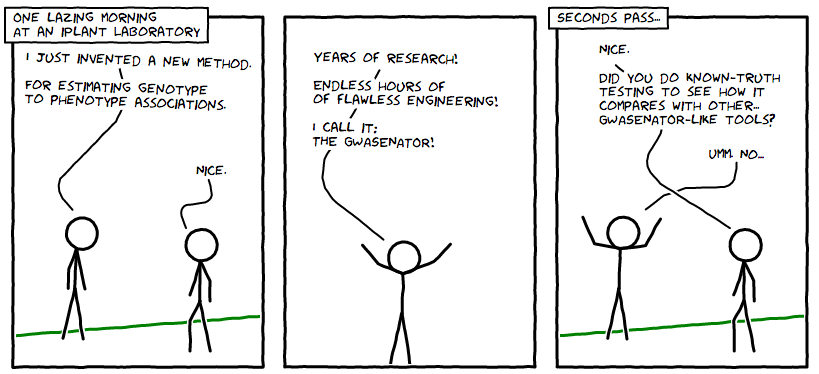
\includegraphics[width=17cm]{doc_comic1}}
\end{center}

\section{Introduction}

\subsection{About the Developers}

\marginlabel{Project Lead and Principal Investigator}Dr. Ann Stapleton works at the interfaces, such as the junctions between research and teaching, individual research projects and large collaborative projects, the organization of international meetings and high-school teacher inquiry labs. Most recently, she has worked at the interface between plant biology and software engineering, leading the way to broad methods applicable to evaluating genotype-to-phenotype analytical methods.

\marginlabel{Statistical Analyst and Developer}Dustin Landers received a BS from Appalachian State where he learned a lot about survey research and using statistics to solve problems and answer questions. He continued his education at UNCW by studying Applied Statistics. Moving from world of polling and survey statistics to the that of Big Data, he has an interest in bridging the gap between statistics and software engineering and seeing the combined discipline brought to bear on problems once considered impossible.

\index{author}

\subsection{Why Validate?}

To test known-truth data sets, we had the idea of looking at a bunch of ROC plots for each simulation run in testing a certain tool. Of course, this was never really feasible because any one simulation run could be atypical. We asked ourselves how could we run lots of simulations through a tool, and test the outputs in a way that gave us insight in to the performance of these GWAS and QTL tools?

It was obvious to us that iPlant gave us the resources to make this happen, but we had to make this as easy as possible if we expected people to use it. 

We sought after summary measures of performance in order to break down the complexity of any individual simulation. We ultimately decided on several classification measures such as the area under the ROC curve, H, and the Kolmogorov-Smirnov statistic. For evaluating effect sizes, we include root mean squared error and mean absolute error. 

But how do we run all these simulations? How do we store them all in a single location so we can calculate these measures? How do we visualize them?

These are the problems we sought to solve. For each problem, we have our own solution. We also left them divided. This way you can decide whether to use our solution or to use your own if you have a unique scenario.

\subsection{How to Use This Manual}

Evaluating a GWAS/QTL tool with Validate is essentially three major steps after your application is installed on either the iPlant Foundation API or the Agave API:

\begin{enumerate}
\item \textbf{Running the Tool With Simulations As Inputs.}
\seealso{Section 2}
This step involves deciding what simulations to use and then iterating over those simulations and submitting them as job requests through the API. We recommend using some sort of scripting method that you are comfortable with. At this point, we don't have a standalone application for submitting jobs. We use rPlant, which is freely available R package that allows you to connect with iPlant's API layer to submit job requests. We also recommend sampling about 300-500 simulations per tool tested.
\item \textbf{Aggregating the Outputs into a Single Folder.}
\seealso{Section 3}
This part is a bit of a logistical exercise. You need to put all your tool outputs that you want to be analyzed using the same known-truth metadata in to aggregate folders. For example, say we are using simulations that are generated using varying levels of heritability. Since the varying heritability values in essence produce different SNP effects, we need to essentially run Validate three separate times. Validate requires an input on an entire folder, and then iterates over those tool outputs. So the first step here, is to decide how many different runs we need to do and then create that many folders. We provide a GUI tool, \textit{Aggregate} that allows you to select files from multiple folders on your iPlant data store (multiple runs of a single tool) and move those (or aggregate them) in to a single folder.
\item \textbf{Running \textit{Validate} on the Aggregated Folder.}
\seealso{Section 4}
Once you have all your outputs in aggregated folders. You can simply log in to the iPlant Discovery Environment and run \textit{Validate} on that folder. You must know two column names in the outputs: The name of the SNP column, and the name of threshold column (such as P-value). Further, if you wish the get back effect size estimation errors, you must also know the column on the estimated effect size column (for example, PLINK's is BETA). Once you submit Validate, you will receive a notification when it is completed. The \textit{Validate} output will be columns of performance measures for each tool output.
\item \textbf{Running \textit{Demonstrate} on the Validate Output.}
\seealso{Section 5}
\end{enumerate}

\section{Running Simulations}

\index{layout design}

\subsection{How To Run Simulations}
\index{rules}

\subsection{PLINK: An Example}

%%%%%%%%%%%%%%%%%%%%%%%%%%%%%%%%%%%%%%%%%%%%%%%%%%%%%%%%%%%%%%%%%%%%%%

\section{Aggregating with Aggregate}
\label{layout}

\subsection{How to Use Aggregate}

\subsection{Continuing our Example}

\section{Validating with Validate}

\subsection{How to Use Validate}

\subsection{Validating PLINK: An Example}

\section{Visualizing the Validation}

\subsection{How to Use the Demonstrate R Package}

\subsection{Demonstrating the Validation of PLINK: An Example}

\end{document}